%%%%%%%%%%%%%%%%%%%%%%%%%%%%%%%%%%%%%%%%%
% Programming/Coding Assignment
% LaTeX Template
%
% This template has been downloaded from:
% http://www.latextemplates.com
%
% Original author:
% Ted Pavlic (http://www.tedpavlic.com)
%
% Note:
% The \lipsum[#] commands throughout this template generate dummy text
% to fill the template out. These commands should all be removed when 
% writing assignment content.
%
% This template uses a Perl script as an example snippet of code, most other
% languages are also usable. Configure them in the "CODE INCLUSION 
% CONFIGURATION" section.
%
%Assignment 2
%Author Zetan
%%%%%%%%%%%%%%%%%%%%%%%%%%%%%%%%%%%%%%%%%

%----------------------------------------------------------------------------------------
%	PACKAGES AND OTHER DOCUMENT CONFIGURATIONS
%----------------------------------------------------------------------------------------

\documentclass{article}

\usepackage{fancyhdr} % Required for custom headers
\usepackage{lastpage} % Required to determine the last page for the footer
\usepackage{extramarks} % Required for headers and footers
\usepackage[usenames,dvipsnames]{color} % Required for custom colors
\usepackage{graphicx} % Required to insert images
\usepackage{listings} % Required for insertion of code
\usepackage{courier} % Required for the courier font
\usepackage{lipsum} % Used for inserting dummy 'Lorem ipsum' text into the template
\usepackage{url}

% Margins
\topmargin=-0.45in
\evensidemargin=0in
\oddsidemargin=0in
\textwidth=6.5in
\textheight=9.0in
\headsep=0.25in

\linespread{1.1} % Line spacing

% Set up the header and footer
\pagestyle{fancy}
\lhead{\hmwkAuthorName} % Top left header
\chead{\hmwkClass\ (\hmwkClassInstructor\ \hmwkClassTime): \hmwkTitle} % Top center head
\rhead{\firstxmark} % Top right header
\lfoot{\lastxmark} % Bottom left footer
\cfoot{} % Bottom center footer
\rfoot{Page\ \thepage\ of\ \protect\pageref{LastPage}} % Bottom right footer
\renewcommand\headrulewidth{0.4pt} % Size of the header rule
\renewcommand\footrulewidth{0.4pt} % Size of the footer rule

\setlength\parindent{0pt} % Removes all indentation from paragraphs

%----------------------------------------------------------------------------------------
%	CODE INCLUSION CONFIGURATION
%----------------------------------------------------------------------------------------

\definecolor{MyDarkGreen}{rgb}{0.0,0.4,0.0} % This is the color used for comments
\lstloadlanguages{Python} % Load python syntax for listings, for a list of other languagesftp://ftp.tex.ac.uk/tex-archive/macros/latex/contrib/listings/listings.pdf supported see: 
\lstset{
        frame=single, % Single frame around code
        basicstyle=\small\ttfamily, % Use small true type font
        keywordstyle=[1]\color{Blue}\bf, % python functions bold and blue
        keywordstyle=[2]\color{Purple}, % python function arguments purple
        keywordstyle=[3]\color{Blue}\underbar, % Custom functions underlined and blue
        identifierstyle=, % Nothing special about identifiers                                         
        commentstyle=\usefont{T1}{pcr}{m}{sl}\color{MyDarkGreen}\small, % Comments small dark green courier font
        stringstyle=\color{Purple}, % Strings are purple
        showstringspaces=false, % Don't put marks in string spaces
        tabsize=5, % 5 spaces per tab
        breaklines=true,
        %
        % Put standard python functions not included in the default language here
        morekeywords={rand},
        %
        % Put python function parameters here
        morekeywords=[2]{on, off, interp},
        %
        % Put user defined functions here
        morekeywords=[3]{test},
       	%
        morecomment=[l][\color{Blue}]{...}, % Line continuation (...) like blue comment
        numbers=left, % Line numbers on left
        firstnumber=1, % Line numbers start with line 1
        numberstyle=\tiny\color{Blue}, % Line numbers are blue and small
        stepnumber=5 % Line numbers go in steps of 5
}

% Creates a new command to include a pyton script, the first parameter is the filename of the script (without .py), the second parameter is the caption
\newcommand{\pythonscript}[2]{
\begin{itemize}
\item[]\lstinputlisting[language=python,caption=#2,label=#1]{#1.py}
\end{itemize}
}
% Creates a new command to include a shell script, the first parameter is the filename of the script (without .sh), the second parameter is the caption
\newcommand{\shellscript}[2]{
\begin{itemize}
\item[]\lstinputlisting[language=bash,caption=#2,label=#1]{#1.sh}
\end{itemize}
}
% Creates a new command to include a R script, the first parameter is the filename of the script (without .R), the second parameter is the caption
\newcommand{\Rscript}[2]{
\begin{itemize}
\item[]\lstinputlisting[language=R,caption=#2,label=#1]{#1.R}
\end{itemize}
}
%----------------------------------------------------------------------------------------
%	DOCUMENT STRUCTURE COMMANDS
%	Skip this unless you know what you're doing
%----------------------------------------------------------------------------------------

% Header and footer for when a page split occurs within a problem environment
\newcommand{\enterProblemHeader}[1]{
\nobreak\extramarks{#1}{#1 continued on next page\ldots}\nobreak
\nobreak\extramarks{#1 (continued)}{#1 continued on next page\ldots}\nobreak
}

% Header and footer for when a page split occurs between problem environments
\newcommand{\exitProblemHeader}[1]{
\nobreak\extramarks{#1 (continued)}{#1 continued on next page\ldots}\nobreak
\nobreak\extramarks{#1}{}\nobreak
}

\setcounter{secnumdepth}{0} % Removes default section numbers
\newcounter{homeworkProblemCounter} % Creates a counter to keep track of the number of problems

\newcommand{\homeworkProblemName}{}
\newenvironment{homeworkProblem}[1][Problem \arabic{homeworkProblemCounter}]{ % Makes a new environment called homeworkProblem which takes 1 argument (custom name) but the default is "Problem #"
\stepcounter{homeworkProblemCounter} % Increase counter for number of problems
\renewcommand{\homeworkProblemName}{#1} % Assign \homeworkProblemName the name of the problem
\section{\homeworkProblemName} % Make a section in the document with the custom problem count
\enterProblemHeader{\homeworkProblemName} % Header and footer within the environment
}{
\exitProblemHeader{\homeworkProblemName} % Header and footer after the environment
}

\newcommand{\problemAnswer}[1]{ % Defines the problem answer command with the content as the only argument
\noindent\framebox[\columnwidth][c]{\begin{minipage}{0.98\columnwidth}#1\end{minipage}} % Makes the box around the problem answer and puts the content inside
}

\newcommand{\homeworkSectionName}{}
\newenvironment{homeworkSection}[1]{ % New environment for sections within homework problems, takes 1 argument - the name of the section
\renewcommand{\homeworkSectionName}{#1} % Assign \homeworkSectionName to the name of the section from the environment argument
\subsection{\homeworkSectionName} % Make a subsection with the custom name of the subsection
\enterProblemHeader{\homeworkProblemName\ [\homeworkSectionName]} % Header and footer within the environment
}{
\enterProblemHeader{\homeworkProblemName} % Header and footer after the environment
}

%----------------------------------------------------------------------------------------
%	NAME AND CLASS SECTION
%----------------------------------------------------------------------------------------

\newcommand{\hmwkTitle}{Assignment\ \#2} % Assignment title
\newcommand{\hmwkDueDate}{Thursday,\ February\ 11,\ 2016} % Due date
\newcommand{\hmwkClass}{Web Science\ cs532} % Course/class
\newcommand{\hmwkClassTime}{4:20pm} % Class/lecture time
\newcommand{\hmwkClassInstructor}{Dr.Michael.L.Nelson} % Teacher/lecturer
\newcommand{\hmwkAuthorName}{Zetan Li} % Your name

%----------------------------------------------------------------------------------------
%	TITLE PAGE
%----------------------------------------------------------------------------------------

\title{
\vspace{2in}
\textmd{\textbf{\hmwkClass:\ \hmwkTitle}}\\
\normalsize\vspace{0.1in}\small{Due\ on\ \hmwkDueDate}\\
\vspace{0.1in}\large{\textit{\hmwkClassInstructor\ \hmwkClassTime}}
\vspace{3in}
}

\author{\textbf{\hmwkAuthorName}}
\date{} % Insert date here if you want it to appear below your name

%----------------------------------------------------------------------------------------

\begin{document}

\maketitle

%----------------------------------------------------------------------------------------
%	TABLE OF CONTENTS
%----------------------------------------------------------------------------------------

%\setcounter{tocdepth}{1} % Uncomment this line if you don't want subsections listed in the ToC

\newpage
\tableofcontents
\newpage

%----------------------------------------------------------------------------------------
%	PROBLEM 1
%----------------------------------------------------------------------------------------

% To have just one problem per page, simply put a \clearpage after each problem

\begin{homeworkProblem}
Write a Python program that extracts 1000 unique links from
Twitter.  You might want to take a look at:\\
\\
\url{http://thomassileo.com/blog/2013/01/25/using-twitter-rest-api-v1-dot-1-with-python/}\\
\\
But there are many other similar resources available on the web.  Note
that only Twitter API 1.1 is currently available; version 1 code will
no longer work.\\
\\
Also note that you need to verify that the final target URI (i.e., the
one that responds with a 200) is unique.  You could have many different
shortened URIs for \url{www.cnn.com} (\url{t.co, bit.ly},\url{goo.gl}, etc.).\\
\\
You might want to use the search feature to find URIs, or you can
pull them from the feed of someone famous (e.g., Tim O'Reilly).\\
\\
Hold on to this collection -- we'll use it later throughout the semester.\\

\centerline{SOLUTION}
To extract urls from twitter, we should get access to twitter API first. After register a twitter application, run the script to get the authentication code.\cite{mytweet}
\\
\pythonscript{mytweets}{python script to get authentication code}
After getting access code, we can use that to get urls from twitter.\\
To achieve this ,we want to use stream listener to get the tweet from twitter and extract link in them, this is the faster way than search method.\cite{extract_link}\\
(the sys.out line is to print work progress on the screen)
\pagebreak
\pythonscript{geturl}{python script to extract urls from tweets}
Note that not all tweets have url in them and many urls we get are duplicates to each other. So the tweets without ulrs are ought to be dropped. And we should extract more than 1000 urls for there are many duplicated links. Here, 10k raw links are extracted for later use.\\
\\
Next step is to extract 1000 unique valid links from raw data. In python \textbf{set} can fulfill that need. For url validating, \textbf{requests} module is a nice tool for that, the link that received 200 response or the final redirected link with 200 response is left in the list.\\
\pagebreak
\pythonscript{unique_url}{python script to get unique\&valid urls}
\end{homeworkProblem}
\newpage
%----------------------------------------------------------------------------------------
%	PROBLEM 2
%----------------------------------------------------------------------------------------

\begin{homeworkProblem}
Download the TimeMaps for each of the target URIs.  We'll use the ODU 
Memento Aggregator, so for example:\\
\\
URI-R = \url{http://www.cs.odu.edu/}\\
\\
URI-T = \url{http://mementoproxy.cs.odu.edu/aggr/timemap/link/1/http://www.cs.odu.edu/}\\
\\
Create a histogram* of URIs vs. number of Mementos (as computed from
the TimeMaps).  For example, 100 URIs with 0 Mementos, 300 URIs
with 1 Memento, 400 URIs with 2 Mementos, etc.\\
\centerline{SOLUTION}
Instead of use python, shell script is used for this problem. With shell, we can access curl's output directly. Then filter out memento links and check time map links by pipeline the out put into grep.
\shellscript{momento}{Shell script for counting memento and recursively check time map}
Once we get the data, it is written in ``url memento" format. The symbols in url will trigger error in data importing in R. So a script is written to keep only memento numbers in the data list.
\shellscript{convertToR}{Convert the data to safe format for R}
Below is the R code to plot histogram of the data. Since the url with zero memento is far more than others, y axis value is scaled by log10.\\
* We add 1 to each y value to avoid log10(0) calculation, for this will result in -infinity and make a hole in the graph.
\Rscript{a2}{R script for histogram}
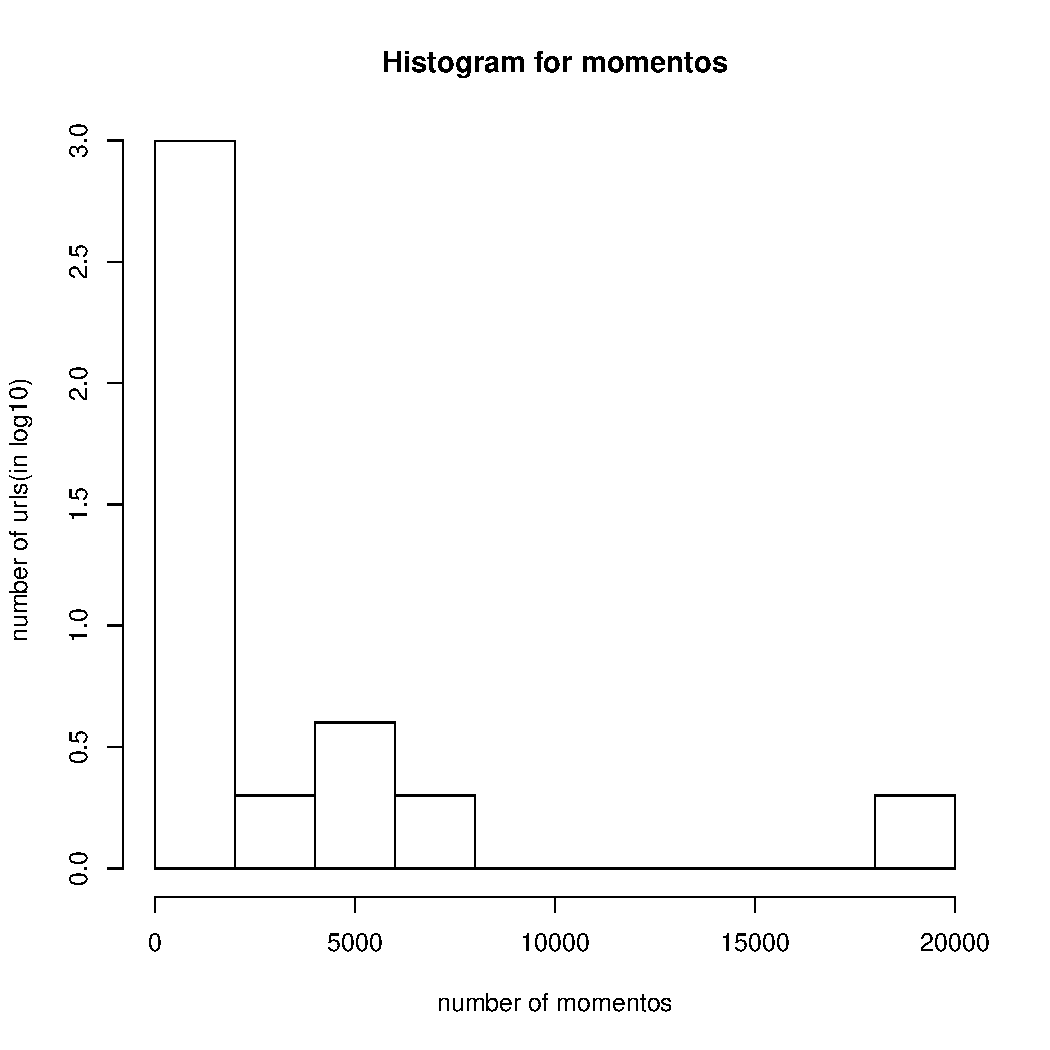
\includegraphics{momento_plot}
\end{homeworkProblem}
\newpage
%----------------------------------------------------------------------------------------
%	PROBLEM 3
%----------------------------------------------------------------------------------------

\begin{homeworkProblem}
Estimate the age of each of the 1000 URIs using the ``Carbon Date" tool:\\
\\
\url{http://ws-dl.blogspot.com/2014/11/2014-11-14-carbon-dating-web-version-20.html}\\
\\
Note: you'll should download the library and run it locally; don't
try to use the web service.\\
\\
For URIs that have > 0 Mementos and an estimated creation date,
create a graph with age (in days) on one axis and number of mementos
on the other.  \\
\\
Not all URIs will have Mementos, and not all URIs will have an estimated
creation date.  State how many fall into either categories. \\
\centerline{SOLUTION}
Since we have data files in problem 2. We want to push these url with mementos greater than 0 into carbon date tool and filter out those have no estimated birth date to get the final data. \\
\\
Below is the code to get the carbon date of urls that have memento numbers greater than 0. We import the local.py as module, and re-parsing the string formatted result to a json object. Then we can retrieve the ``Estimated carbon date'' value out of the object.\\
\\
Note that this script must be run under carbon date tool directory.
\pythonscript{a3}{Python code to get carbon date}
\pagebreak
Then plot these data into scatter graph.
\Rscript{a3}{R script to plot scatter graph}
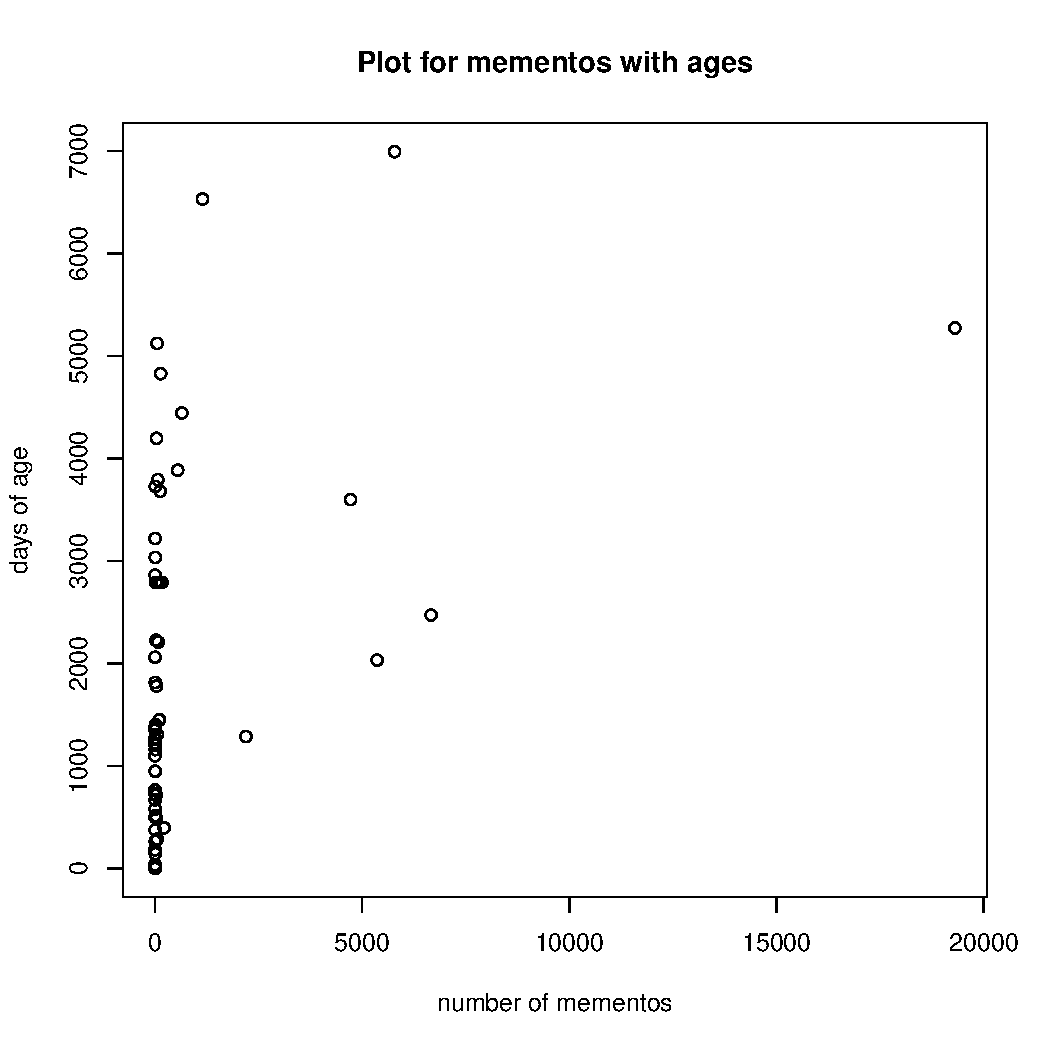
\includegraphics{age_plot}
\end{homeworkProblem}
\pagebreak
\bibliographystyle{plain}
\bibliography{ref}
\end{document}